% =====================================================================
%  Chapter 4 — The Mathematics, Part II
% =====================================================================

\chapter{Four Obstacles}
\label{ch:barriers}

Chapter~3 said what must be proved. This chapter says what makes it hard, and
it does so by taking seriously the four places where the proposed method runs
into a wall. Each wall is a wall that has stopped somebody before, and three
of the four are still standing in the literature today.

This is not a list of objections to the claim. It is the background against
which the claim has to be read, and it is the background that makes the
remaining argument in Chapter~5 interpretable.

\section{The function-field barrier}\subsection{The method that worked}Over a finite field $\FF_q$, the Riemann hypothesis for the zeta function of
the curve $C/\FF_q$ was proved independently by Weil (using his theory of
Frobenius correspondences) and by Stepanov (using an elementary method, and
with a decisive contribution to the theory of algebraic curves over finite
fields), with Bombieri giving the clean modern presentation.

The Stepanov--Bombieri method\idx{Stepanov--Bombieri method} is, in outline: choose a cleverly chosen divisor
or a system of hyperplane sections on $C$; consider the divisor
\begin{equation}
D = \sum_{i=1}^{r} (D_i) \quad\text{with}\quad D_i \text{ of the form }
       (m_i + n_i g) \text{ on a hyperplane section},
\label{eq:stepanov}
\end{equation}
where $g$ is a function on $C$; observe that the linear system of functions
with poles bounded by $D$ has dimension determined by the geometry of $C$; and
deduce from a dimension count that some function in the system has a zero of
high multiplicity, or that the number of points of $C$ is bounded.

Two features of this argument are decisive, and both are about \emph{dimension}.

\begin{quote}
\textbf{First: two directions.} A curve over a finite field is a
\emph{geometric} object, but the counting is \emph{arithmetic} --- it counts
$\FF_q$-points, hence the $q$-power growth. The method exploits the product of
these two: the geometry supplies a dimension count, and the arithmetic
supplies the growth rate. Formally, the product $\operatorname{Spec}\FF_q
\times \operatorname{Spec}\FF_q$ is two-dimensional, and a divisor with
multiplicity $m$ on one factor contributes $m$ times the dimension of the
other.

\textbf{Second: multiplicity.} The dimension count works best when the
divisor has high multiplicity, and high multiplicity is available because the
geometric factor contributes $\dim H^0$ of a line bundle raised to a power.
This is the ``divisor involving multiplicity'' that the remark refers to.
\end{quote}

\subsection{Why it does not transfer}Over $\ZZ$, the arithmetic factor is $\operatorname{Spec}\ZZ$. The product
$\operatorname{Spec}\ZZ \times \operatorname{Spec}\ZZ$ is \emph{one}-dimensional:
it is $\operatorname{Spec}\ZZ$. There is no second direction, so no second
factor to multiply a dimension count by, and the argument loses exactly the
multiplicity that made it work.

This is not a technical inconvenience. Maarten van Frankenhuijsen\idx{van Frankenhuijsen, Maarten}'s note
\emph{The Riemann Hypothesis for Function Fields over a Finite Field}
(arXiv:0806.0044) states the situation directly: the Stepanov and Bombieri
methods both require the product $C \times C$ of a geometric curve with an
arithmetic curve, one coordinate geometric and one arithmetic, and the methods
``do not work over $\ZZ$'' because there the analogous product collapses to a
single copy of $\operatorname{Spec}\ZZ$.

The remark's author knows this precisely. His formulation of the problem is
that multiplicity is ``hard to find over the integers, corresponding to
something like differentiating whole numbers''. He is asking for a way to
manufacture multiplicity in a one-dimensional arithmetic setting.

\begin{deeper}{What a substitute for multiplicity would have to do}
Suppose we want to prove RH over $\ZZ$ by the Stepanov--Bombieri route. We need
a space of functions $f$ on some arithmetic geometric object, with a bound on
the poles of $f$ controlled by a divisor $D$, such that the dimension of that
space grows fast enough to force a high-multiplicity zero. Over a finite field
the growth rate $q^{\dim}$ comes from the arithmetic side.

There are exactly two plausible sources of such growth over $\ZZ$: the
\emph{analytic} growth of a space of modular forms (theta series, whose
coefficients are exponential in the weight), and the \emph{cohomological}
growth of a tower of class groups or an Iwasawa tower (where the growth comes
from the degree of the tower rather than from a finite field). The remark
proposes both --- iterated theta lifts for the analytic growth, Iwasawa towers
``specifically using Behrend'' for the cohomological growth --- and the whole
structure of the argument is the attempt to make them pay for each other.

This is why the submission's dependency chain passes through Siegel--Weil
formula data, theta lift existence, and Iwasawa decomposition machinery. It
is also why the fidelity of those inputs is the thing to check: they are where
the growth is supposed to come from.
\end{deeper}

\section{The automorphy gap}\subsection{What the method needs}To make a theta lift do the work of a multiplicity, one needs to know that the
lifted object is something well-behaved --- in practice, that it is
\emph{automorphic}: that it arises from an automorphic form, and hence that its
$L$-function is a genuine $L$-function with the analytic properties one needs.

The remark's timeline describes the intended mechanism. Item 3 notes that
``$\mu$ is automorphic from $\theta$ on sixfold cover of GL$_5$ as a period
integral of thetas''; item 16 invokes the ``Relative trace formula'' to get
``automorphy of $\mu$ and reducing via Cauchy--Schwartz to a bound on the norm
of a suitably projected Poincar\'e series''; item 8 chains lifts
$U(X_0) \to U(X_1) \to \cdots \to U(X_m)$ between totally definite unitary
groups.

\subsection{What is known}Here the honest answer is uncomfortable, and it is the sort of thing that
press coverage tends to round off.

\begin{itemize}
\item The theorem that is actually proved in general for unitary groups is
\textbf{Gross--Prasad}\idx{Gross--Prasad theorem}, not ``Gross--Petersson'' as it is often misattributed.
\item Even the Gross--Prasad theorem is proved in the \emph{unitary} case. The
corresponding \emph{orthogonal} case remains open in general.
\item More specifically: no general theorem establishing \emph{both}
automorphy and analyticity of the third-place theta lift was located in the
primary literature. The specific third-place lift that the method needs has
no primary record at all.
\end{itemize}

That last point is the crux, and it needs stating carefully so that it is not
over- or under-stated.

\begin{seamnote}{What is and is not claimed here}
This book does \emph{not} claim that the automorphy step of the submitted proof
is wrong. It does not claim the author has made an error. What it records is
that the step is, in the literature, an open problem in the generality the
remark requires, and that no published result covers it.

The alternative is equally unattractive and must be named: the step might be
discharged by something the author has proved and not yet published --- which
is exactly what the Lean development is supposed to contain. Chapter~8 examines
the formalized statement of that step, \texttt{Af.NewformAut}, and Chapter~14
sets out how to check it.

So the situation is: a known open problem, or an unpublished proof of it. Both
are possible. Only one of them is a proof of RH.
\end{seamnote}

\section{The surviving classes, and Vandiver}The remark's item 17 is the most technical and the least explicated of its
twenty entries:

\begin{quote}
\small
``for the classes in $H^1_o\idx{H\textsuperscript{1}o classes}(\QQ_\ell/\ZZ_\ell(-e))$ that we couldn't kill by
twisting, fight for a significant weakening of Vandiver.''
\end{quote}

The mechanism being invoked is standard in the theory of modular forms and
Iwasawa theory: one kills unwanted cohomology classes by twisting with
characters, using the fact that a non-trivial character is orthogonal to
everything. What survives the twisting is the obstruction, and what survives is
what the remark calls the $H^1_o$ classes --- the part of $H^1$ that is
``obstruction-like'' in the Iwasawa-theoretic sense.

The proposed remedy is a ``significant weakening of Vandiver''.

\begin{quote}
\textbf{Vandiver's conjecture}\idx{Vandiver's conjecture} asserts that the class group of the maximal real
subfield of a cyclotomic field has odd part trivial: more precisely, that the
plus part of the class group of $\QQ(\zeta_m)^+$ has odd order for all $m$.
It is known to be true for a great many individual $m$; it is verified
computationally for all $m$ with $\varphi(m)$ below $2^{31}$, a result of Hart,\idx{Hart--Harvey--Ong bound}
Harvey and Ong published in \emph{Mathematics of Computation} \textbf{86}
(2017), 3031--3049 (DOI 10.1090/mcom/3211, arXiv:1605.02398).

\textbf{Vandiver's conjecture remains open.}
\end{quote}

This is a genuine red flag, for two reasons that compound.

\begin{enumerate}
\item A weakening of Vandiver is a \emph{new conjecture}. Nobody has proved a
significant weakening of Vandiver. If the argument needs one, the argument
needs something that does not exist.
\item The footnote to the remark's item 17 says: ``This is still pretty strong!!
I believe vanishing of a number of $K$-groups of $\ZZ$ follows, and cyclicity
up to 100ish maybe?'' The register --- exclamation marks, ``maybe?'' --- is
not the register of a settled step. It is the register of a hope.
\end{enumerate}

Compare item 19, ``precise choice of the Iwasawa tower, specifically using
Behrend'', whose footnote says ``This is the sort of trick that intuitively to
me is obviously going to be unnecessary.'' The author's own footnotes mark the
places where the argument is doing something the author does not fully
control.

\section{The two-thirds ceiling}And now the wall that this book takes most seriously, because it is not a wall
that somebody else hit: it is one the author hit and recorded.

The remark's item 14 reads, in full:

\begin{quote}
\small
``precise computation of the `cost' of each lift, showing that one would stop at
2/3 a priori, attempt to get a main term and transfer constant to a function
field or kill via twisting, need for `division'.''
\end{quote}

Parse it as a sequence of events on 15 November 2026.

\begin{enumerate}
\item A computation was carried out of the cost of each theta lift.
\item The result was that the method \emph{would stop at two thirds a priori}\idx{two-thirds ceiling}.
That is: the analytic cost of building the required chain of lifts eats more
than one third of the available multiplicity, and the method as then
understood yields a bound covering two thirds of the zeros, not all of them.
\item The response was an \emph{attempt}: ``attempt to get a main term and
transfer constant to a function field or kill via twisting, need for
`division'.''
\end{enumerate}

And then, the following day, item 20: ``11/16/26: GRH.''

\begin{seamnote}{Why the ceiling matters more than it might appear}
Two thirds is not an arbitrary number. It is, almost exactly, the number the
\emph{same author} had already reached three months earlier with the same
method family --- and that result is a real, published, independently
reproduced, formally verified theorem. Chapter~11 is about it.

So the situation is: on 15 November the method's own author computed that it
stopped at the same place it had stopped in August. On 16 November, GRH was
recorded as established. The remark does not say what changed.

There are only three possibilities, and the book's evidence does not currently
discriminate between them:

\begin{description}[style=nextline,leftmargin=0pt,font=\sffamily\bfseries\small,
  itemsep=5pt]
\item[\textbf{A.}] The Lean development contains a genuine additional
ingredient --- the ``main term'' or the ``division'' or the twist-killing that
item 14 lists as attempts --- which does what the remark's timeline, being a
``slop'' summary, does not describe.
\item[\textbf{B.}] The two-thirds ceiling was a cost accounting that the
author subsequently found to be wrong or avoidable, and the remark records the
older, superseded state.
\item[\textbf{C.}] The formalisation proves something weaker than the
headline theorem, and the headline theorem is obtained by a step that a
reader has not yet checked.
\end{description}

Possibility \textbf{A} would be extraordinary and would settle the matter in
the claim's favour. Possibility \textbf{B} is unremarkable and would also
settle it in the claim's favour. Possibility \textbf{C} would be the standard
failure mode of a formalised proof, and it is the one that a compiler cannot
detect and a reader must.

This is not an accusation. It is the statement of why the audit in Part~III
is necessary, and it is why Chapter~14 is a protocol rather than a verdict on
the mathematics.
\end{seamnote}

\begin{figure}[!htbp]
\centering
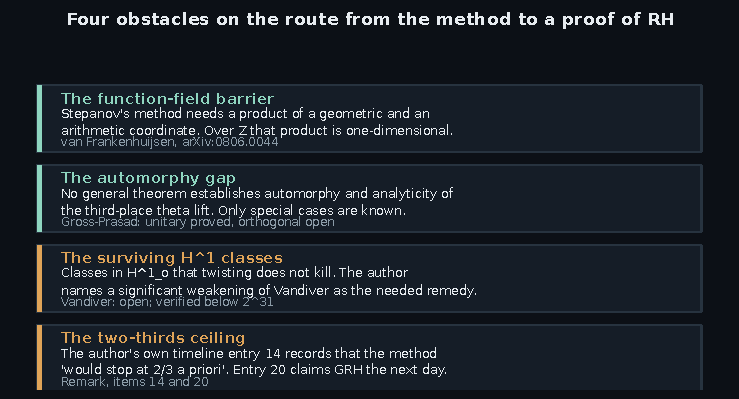
\includegraphics[width=\textwidth]{../figures/fig_barriers.pdf}
\caption{The four obstacles, in the order in which the method encounters them.
The first two are classical walls with a long literature behind them; the third
names an open conjecture as its remedy; the fourth is recorded by the author
himself.}
\label{fig:barriers}
\end{figure}

\section{A note on how strong the walls are}It would be a mistake to read this chapter as an argument that the claim is
implausible. Three qualifications.

\begin{enumerate}
\item \textbf{The first two walls are not proof of impossibility.} The
function-field barrier has been crossed before, in a different direction, by
techniques nobody expected --- Weil's own approach was not Stepanov's. The
theta-lift wall is a wall in the current state of the literature, not a
theorem about what can be proved.
\item \textbf{The artifact is enormous, and scale changes what is plausible.}
At 175{,}187 files and roughly 17.4 million lines, the development contains
room for techniques and lemmas that no reviewer has seen. The remark's
author's earlier two-thirds theorem was itself produced by this kind of
effort.
\item \textbf{And the author's own claim about the fourth wall is that he got
past it.} Item 14 ends with a list of attempts, and item 20 is dated the next
day. An author who believed they had stopped at two thirds would not write
``GRH'' the next day. The most likely reading is that something worked. The
question is whether the Lean development contains it.
\end{enumerate}

\begin{keytakeaways}

\item The Stepanov--Bombieri method works over finite fields because the
product of the geometric and arithmetic coordinates is two-dimensional. Over
$\ZZ$ it is one-dimensional, and the method does not transfer. This is the
structural reason the problem is hard.
\item Automorphy of the required theta lift is, in the generality the remark
needs, an open problem; the unitary Gross--Prasad theorem is proved, the
orthogonal case is not, and no general result on the third-place lift was
located.
\item Item 17 names a significant weakening of Vandiver as its remedy.
Vandiver is open; no such weakening is known; and the remark's own footnote
to that item is hedged with ``maybe?''.
\item Item 14 records that the method ``would stop at 2/3 a priori'' on
15 November, and item 20 records GRH on 16 November, with no account of the
change. That gap is the central open question of this book.
\end{keytakeaways}
